\documentclass{uwstat518}\usepackage[]{graphicx}\usepackage[]{color}
%% maxwidth is the original width if it is less than linewidth
%% otherwise use linewidth (to make sure the graphics do not exceed the margin)
\makeatletter
\def\maxwidth{ %
  \ifdim\Gin@nat@width>\linewidth
    \linewidth
  \else
    \Gin@nat@width
  \fi
}
\makeatother

\definecolor{fgcolor}{rgb}{0.345, 0.345, 0.345}
\newcommand{\hlnum}[1]{\textcolor[rgb]{0.686,0.059,0.569}{#1}}%
\newcommand{\hlstr}[1]{\textcolor[rgb]{0.192,0.494,0.8}{#1}}%
\newcommand{\hlcom}[1]{\textcolor[rgb]{0.678,0.584,0.686}{\textit{#1}}}%
\newcommand{\hlopt}[1]{\textcolor[rgb]{0,0,0}{#1}}%
\newcommand{\hlstd}[1]{\textcolor[rgb]{0.345,0.345,0.345}{#1}}%
\newcommand{\hlkwa}[1]{\textcolor[rgb]{0.161,0.373,0.58}{\textbf{#1}}}%
\newcommand{\hlkwb}[1]{\textcolor[rgb]{0.69,0.353,0.396}{#1}}%
\newcommand{\hlkwc}[1]{\textcolor[rgb]{0.333,0.667,0.333}{#1}}%
\newcommand{\hlkwd}[1]{\textcolor[rgb]{0.737,0.353,0.396}{\textbf{#1}}}%

\usepackage{framed}
\makeatletter
\newenvironment{kframe}{%
 \def\at@end@of@kframe{}%
 \ifinner\ifhmode%
  \def\at@end@of@kframe{\end{minipage}}%
  \begin{minipage}{\columnwidth}%
 \fi\fi%
 \def\FrameCommand##1{\hskip\@totalleftmargin \hskip-\fboxsep
 \colorbox{shadecolor}{##1}\hskip-\fboxsep
     % There is no \\@totalrightmargin, so:
     \hskip-\linewidth \hskip-\@totalleftmargin \hskip\columnwidth}%
 \MakeFramed {\advance\hsize-\width
   \@totalleftmargin\z@ \linewidth\hsize
   \@setminipage}}%
 {\par\unskip\endMakeFramed%
 \at@end@of@kframe}
\makeatother

\definecolor{shadecolor}{rgb}{.97, .97, .97}
\definecolor{messagecolor}{rgb}{0, 0, 0}
\definecolor{warningcolor}{rgb}{1, 0, 1}
\definecolor{errorcolor}{rgb}{1, 0, 0}
\newenvironment{knitrout}{}{} % an empty environment to be redefined in TeX

\usepackage{alltt}
\usepackage{graphicx,amssymb,amstext,amsmath,color,verbatim, natbib,setspace}
\usepackage{natbib}
\usepackage{float}
\usepackage{wasysym}
\usepackage{subfig}
\usepackage{tikz}
%\usepackage{hyperref}
%\usepackage[all]{hypcap}
\graphicspath{{converted_graphics/}}
\usepackage{natbib}          % for author year citations \citet \citep
\bibliographystyle{plainnat} % 'plain' will be fine for many purposes
%---------------------------------------------------------
\tikzset{
  invisible/.style={opacity=0},
  visible on/.style={alt=#1{}{invisible}},
  alt/.code args={<#1>#2#3}{%
    \alt<#1>{\pgfkeysalso{#2}}{\pgfkeysalso{#3}} % \pgfkeysalso doesn't change the path
  },
}
\newcommand{\bs}{\boldsymbol}
\newcommand{\sesq}{\sigma_{\epsilon}^{2}}
\newcommand{\ssq}{\sigma^{2}}
\newcommand{\e}{\epsilon}
\newcommand{\E}{\text{E}}
\newcommand{\Var}{\text{Var}}
\newcommand{\Cov}{\text{Cov}} \newcommand{\logit}{\text{logit}}
\newcommand{\mN}{\mathcal{N}}
\newcommand{\mX}{\mathcal{X}}
         % for author year citations \citet \citep
\renewcommand{\baselinestretch}{1}
\usepackage{titling}
\setlength{\droptitle}{-1in}
\usepackage{url}
\IfFileExists{upquote.sty}{\usepackage{upquote}}{}
\begin{document}
\title{Comparison of two versions of turnover constraint optimization}
\author{Kirk Li}
\maketitle
\section{source scripts, load data}

\begin{knitrout}
\definecolor{shadecolor}{rgb}{0.969, 0.969, 0.969}\color{fgcolor}\begin{kframe}
\begin{alltt}
\hlcom{# global chunk options}
\hlkwd{library}(knitr)
opts_chunk$\hlkwd{set}(cache = TRUE, tidy = FALSE, autodep = TRUE, fig.width = 6, fig.height = 6)
\end{alltt}
\end{kframe}
\end{knitrout}


\begin{knitrout}
\definecolor{shadecolor}{rgb}{0.969, 0.969, 0.969}\color{fgcolor}\begin{kframe}
\begin{alltt}
inslib <- \hlkwd{function}(x)\{
	x <-\hlkwd{as.character}(\hlkwd{substitute}(x))
	\hlkwd{if}(!x %in% \hlkwd{rownames}(\hlkwd{installed.packages}())) 
	\{\hlkwd{install.packages}(x)\}
	\hlkwd{eval}(\hlkwd{parse}(text=\hlkwd{paste}(\hlstr{"\hlkwd{library}("},x,\hlstr{")"},sep=\hlstr{""})))\}
\hlkwd{inslib}(\hlstr{"quadprog"})
\hlkwd{inslib}(\hlstr{"xts"})
\hlkwd{inslib}(\hlstr{"corpcor"})
\hlkwd{inslib}(knitr) # inslib works w/ "
\hlkwd{source}(\hlstr{"turnoveroptdoug.r"})
\hlkwd{source}(\hlstr{"TurnoverOpt.R"})
\hlkwd{source}(\hlstr{"mvo.constrained.r"})
\hlkwd{source}(\hlstr{"efront.constrained.r"})
\hlkwd{source}(\hlstr{"barplot.wts.r"})
\hlkwd{load}(\hlstr{"crsp.short.Rdata"})
returns = midcap.ts[,1:5]
returns = \hlkwd{coredata}(returns)
\end{alltt}
\end{kframe}
\end{knitrout}


\section{scenario 1: without mean constraints, with shorting allowed:}
\begin{knitrout}
\definecolor{shadecolor}{rgb}{0.969, 0.969, 0.969}\color{fgcolor}\begin{kframe}
\begin{alltt}
mu.target = NULL
long.only = FALSE
toc=turnover=0.2
wts.initial=w.initial=\hlkwd{rep}(1/\hlkwd{ncol}(returns),\hlkwd{ncol}(returns))
res1 <- \hlkwd{TurnoverOpt_doug}(returns, mu.target =mu.target, 
		wts.initial = wts.initial, toc = toc,long.only=long.only)
res2 <- \hlkwd{TurnoverOpt}(returns,mu.target=mu.target, 
		w.initial=wts.initial,turnover=turnover,long.only=long.only)
RES <- \hlkwd{rbind}(\hlkwd{c}(res1$wts,res1$port.mu,res1$port.var,res1$turnover), 
		\hlkwd{c}(res2$w,res2$port.mu, res2$port.var, res2$achieved.turnover))
\hlkwd{colnames}(RES) <- \hlkwd{c}(\hlkwd{rep}(\hlstr{"wt"},5),\hlstr{"mu"},\hlstr{"var"},\hlstr{"turnover"})
\hlkwd{rownames}(RES) <- \hlkwd{c}(\hlstr{"doug"},\hlstr{"previous"})
RES	
\end{alltt}
\begin{verbatim}
##           wt     wt     wt     wt  wt      mu      var turnover
## doug     0.2 0.1640 0.1870 0.1490 0.3 0.01100 0.004000      0.2
## previous 0.2 0.1639 0.1875 0.1486 0.3 0.01126 0.004163      0.2
\end{verbatim}
\end{kframe}
\end{knitrout}


\section{scenario 2: without mean constraints, without shorting:}
\begin{knitrout}
\definecolor{shadecolor}{rgb}{0.969, 0.969, 0.969}\color{fgcolor}\begin{kframe}
\begin{alltt}
mu.target = NULL
long.only = TRUE
toc=turnover=0.2
wts.initial=w.initial=\hlkwd{rep}(1/\hlkwd{ncol}(returns),\hlkwd{ncol}(returns))
res1 <- \hlkwd{TurnoverOpt_doug}(returns, mu.target =mu.target, 
		wts.initial = wts.initial, toc = toc,long.only=long.only)
res2 <- \hlkwd{TurnoverOpt}(returns,mu.target=mu.target, 
		w.initial=wts.initial,turnover=turnover,long.only=long.only)
RES <- \hlkwd{rbind}(\hlkwd{c}(res1$wts,res1$port.mu,res1$port.var,res1$turnover), 
		\hlkwd{c}(res2$w,res2$port.mu, res2$port.var, res2$achieved.turnover))
\hlkwd{colnames}(RES) <- \hlkwd{c}(\hlkwd{rep}(\hlstr{"wt"},5),\hlstr{"mu"},\hlstr{"var"},\hlstr{"turnover"})
\hlkwd{rownames}(RES) <- \hlkwd{c}(\hlstr{"doug"},\hlstr{"previous"})
RES	
\end{alltt}
\begin{verbatim}
##           wt     wt     wt     wt  wt      mu      var turnover
## doug     0.2 0.1640 0.1870 0.1490 0.3 0.01100 0.004000      0.2
## previous 0.2 0.1639 0.1875 0.1486 0.3 0.01126 0.004163      0.2
\end{verbatim}
\end{kframe}
\end{knitrout}



\section{scenario 3: with mean constraints, with shorting allowed:}
\begin{knitrout}
\definecolor{shadecolor}{rgb}{0.969, 0.969, 0.969}\color{fgcolor}\begin{kframe}
\begin{alltt}
mu.target = 0.01
long.only = FALSE
toc=turnover=0.5
res1 <- \hlkwd{TurnoverOpt_doug}(returns, mu.target =mu.target, 
		wts.initial = wts.initial, toc = toc, long.only=long.only)
res2 <- \hlkwd{TurnoverOpt}(returns,mu.target=mu.target, 
		w.initial=wts.initial,turnover=turnover,long.only=long.only)

RES <- \hlkwd{rbind}(\hlkwd{c}(res1$wts,res1$port.mu,res1$port.var,res1$turnover),
		\hlkwd{c}(res2$w,res2$port.mu, res2$port.var, res2$achieved.turnover))
\hlkwd{colnames}(RES) <- \hlkwd{c}(\hlkwd{rep}(\hlstr{"wt"},5),\hlstr{"mu"},\hlstr{"var"},\hlstr{"turnover"})
\hlkwd{rownames}(RES) <- \hlkwd{c}(\hlstr{"doug"},\hlstr{"previous"})
RES	
\end{alltt}
\begin{verbatim}
##              wt     wt      wt     wt     wt   mu      var turnover
## doug     0.2370 0.1780 0.06900 0.1020 0.4130 0.01 0.004000      0.5
## previous 0.2366 0.1782 0.06946 0.1023 0.4134 0.01 0.003828      0.5
\end{verbatim}
\end{kframe}
\end{knitrout}



\section{scenario 4: with mean constraints, without shorting: }
\begin{knitrout}
\definecolor{shadecolor}{rgb}{0.969, 0.969, 0.969}\color{fgcolor}\begin{kframe}
\begin{alltt}
mu.target = 0.01
long.only = TRUE
toc=turnover=0.5
res1 <- \hlkwd{TurnoverOpt_doug}(returns, mu.target =mu.target, 
		wts.initial = wts.initial, toc = toc, long.only=long.only)
res2 <- \hlkwd{TurnoverOpt}(returns,mu.target=mu.target, 
		w.initial=wts.initial,turnover=turnover,long.only=long.only)

RES <- \hlkwd{rbind}(\hlkwd{c}(res1$wts,res1$port.mu,res1$port.var,res1$turnover), 
		\hlkwd{c}(res2$w,res2$port.mu, res2$port.var, res2$achieved.turnover))
\hlkwd{colnames}(RES) <- \hlkwd{c}(\hlkwd{rep}(\hlstr{"wt"},5),\hlstr{"mu"},\hlstr{"var"},\hlstr{"turnover"})
\hlkwd{rownames}(RES) <- \hlkwd{c}(\hlstr{"doug"},\hlstr{"previous"})
RES	
\end{alltt}
\begin{verbatim}
##              wt     wt      wt     wt     wt   mu      var turnover
## doug     0.2370 0.1780 0.06900 0.1020 0.4130 0.01 0.004000      0.5
## previous 0.2366 0.1782 0.06946 0.1023 0.4134 0.01 0.003828      0.5
\end{verbatim}
\end{kframe}
\end{knitrout}


\section{efficient frontier plot:}

Here we compare two versions of turnover on efficient frontier plot, using two
different turnover (0.5, 10).
We found there is no difference in two versions. 

\begin{knitrout}
\definecolor{shadecolor}{rgb}{0.969, 0.969, 0.969}\color{fgcolor}\begin{kframe}
\begin{alltt}
sum=1 \hlcom{# full investment }
mu.target=NULL 
w.initial=\hlkwd{rep}(1/n.stocks,n.stocks) 
toc=0.5
digits=4
wts.only=T
mu.min = NULL 
mu.max = NULL 
rf = .003
npoints = 20
wts.plot = T 
printout = F
bar.ylim = \hlkwd{c}(-1,4)
clist <- \hlkwd{c}(\hlstr{"sum"},\hlstr{"turnover"})
list.arg <- \hlkwd{list}(	
			sum=sum,
			toc=toc,
			w.initial=w.initial)
cset <- NULL
cset <-\hlkwd{combine.cset}(clist=clist,returns=returns,list.arg)
\end{alltt}
\begin{verbatim}
## sum 
## turnover
\end{verbatim}
\begin{alltt}
\hlkwd{efrontPlot}(returns, cset, rf = .003, npoints = 20,wts.plot = T,
		bar.ylim = \hlkwd{c}(-1,4),list.arg=list.arg)
\end{alltt}
\begin{verbatim}
## [1] "turnover/propcost constraints reduced the max mean return in efficient frontier plot"
\end{verbatim}
\begin{alltt}
\hlkwd{mtext}(\hlkwd{paste}(clist,collapse=\hlstr{"_"}),side=1,line=3)
\end{alltt}
\end{kframe}
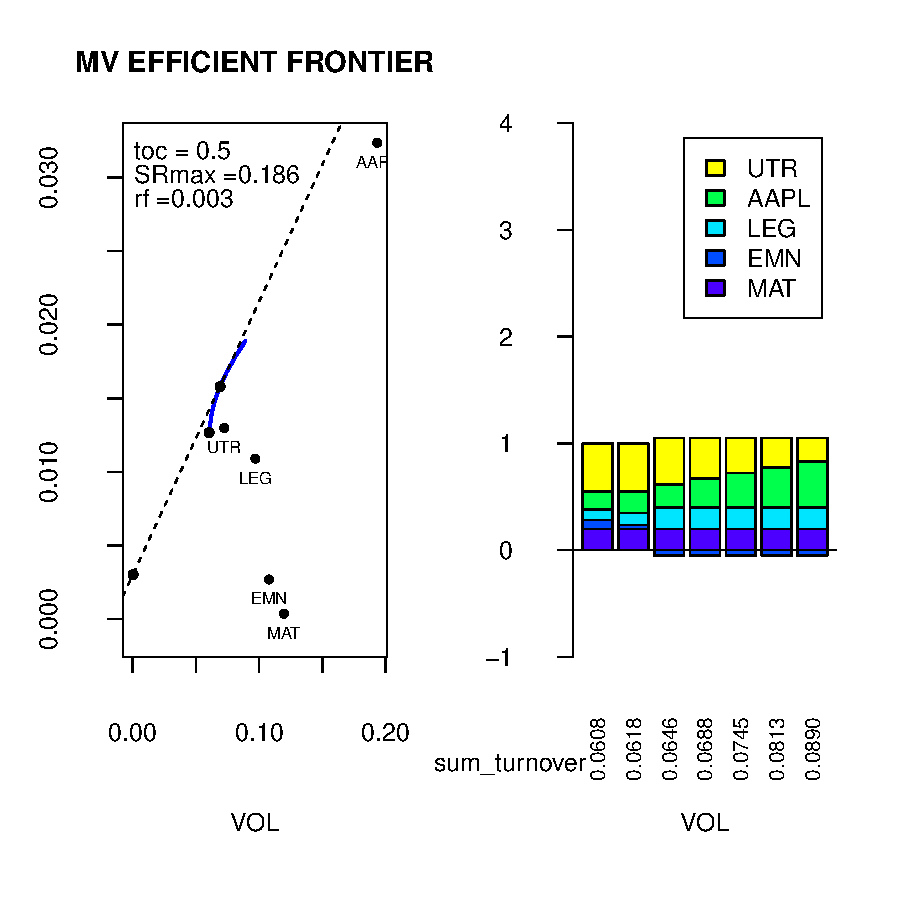
\includegraphics[width=\maxwidth]{figure/unnamed-chunk-61} 
\begin{kframe}\begin{alltt}


clist <- \hlkwd{c}(\hlstr{"sum"},\hlstr{"turnover.doug"})
list.arg <- \hlkwd{list}(	
		sum=sum,
		toc=toc,
		w.initial=w.initial)
cset <- NULL
cset <-\hlkwd{combine.cset}(clist=clist,returns=returns,list.arg)
\end{alltt}
\begin{verbatim}
## sum 
## turnover.doug
\end{verbatim}
\begin{alltt}

\hlkwd{efrontPlot}(returns, cset, rf = .003, npoints = 20,wts.plot = T,
		bar.ylim = \hlkwd{c}(-1,4),list.arg=list.arg)
\end{alltt}
\begin{verbatim}
## [1] "turnover/propcost constraints reduced the max mean return in efficient frontier plot"
\end{verbatim}
\begin{alltt}
\hlkwd{mtext}(\hlkwd{paste}(clist,collapse=\hlstr{"_"}),side=1,line=3)
\end{alltt}
\end{kframe}
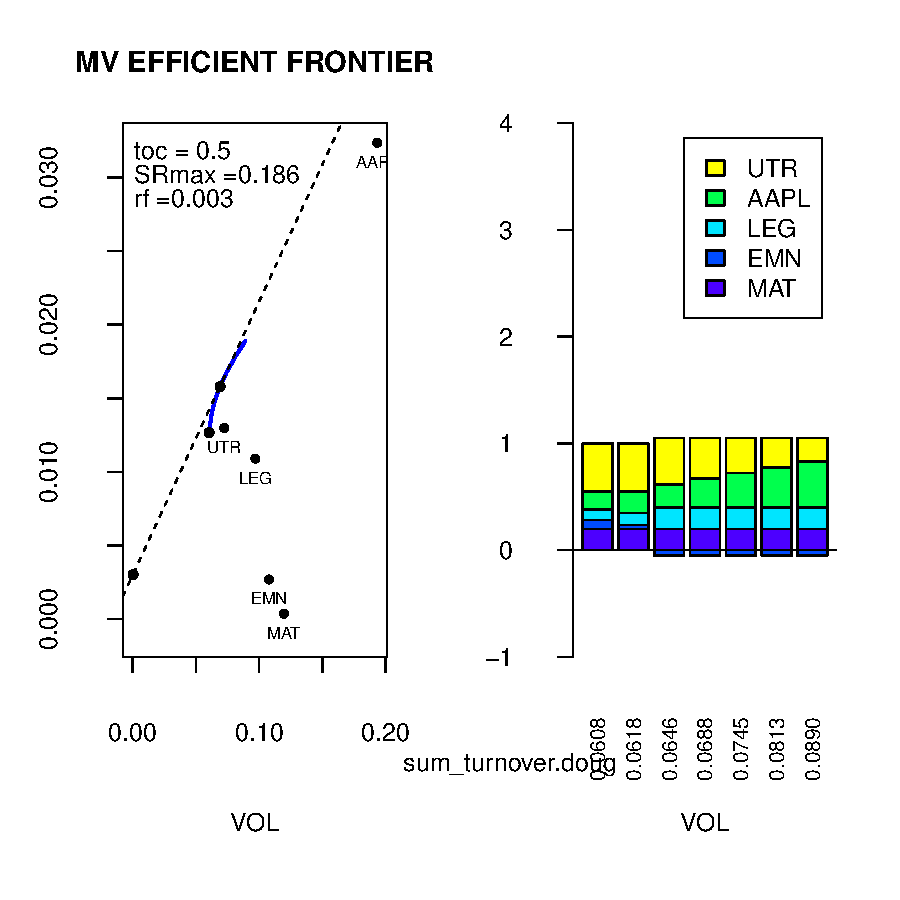
\includegraphics[width=\maxwidth]{figure/unnamed-chunk-62} 

\end{knitrout}


Now we assign a large number toc:
\begin{knitrout}
\definecolor{shadecolor}{rgb}{0.969, 0.969, 0.969}\color{fgcolor}\begin{kframe}
\begin{alltt}
toc=10
clist <- \hlkwd{c}(\hlstr{"sum"},\hlstr{"turnover"})
list.arg <- \hlkwd{list}(	
		sum=sum,
		toc=toc,
		w.initial=w.initial)
cset <- NULL
cset <-\hlkwd{combine.cset}(clist=clist,returns=returns,list.arg)
\end{alltt}
\begin{verbatim}
## sum 
## turnover
\end{verbatim}
\begin{alltt}
\hlkwd{efrontPlot}(returns, cset, rf = .003, npoints = 20,wts.plot = T,
		bar.ylim = \hlkwd{c}(-1,4),list.arg=list.arg)
\hlkwd{mtext}(\hlkwd{paste}(clist,collapse=\hlstr{"_"}),side=1,line=3)
\end{alltt}
\end{kframe}
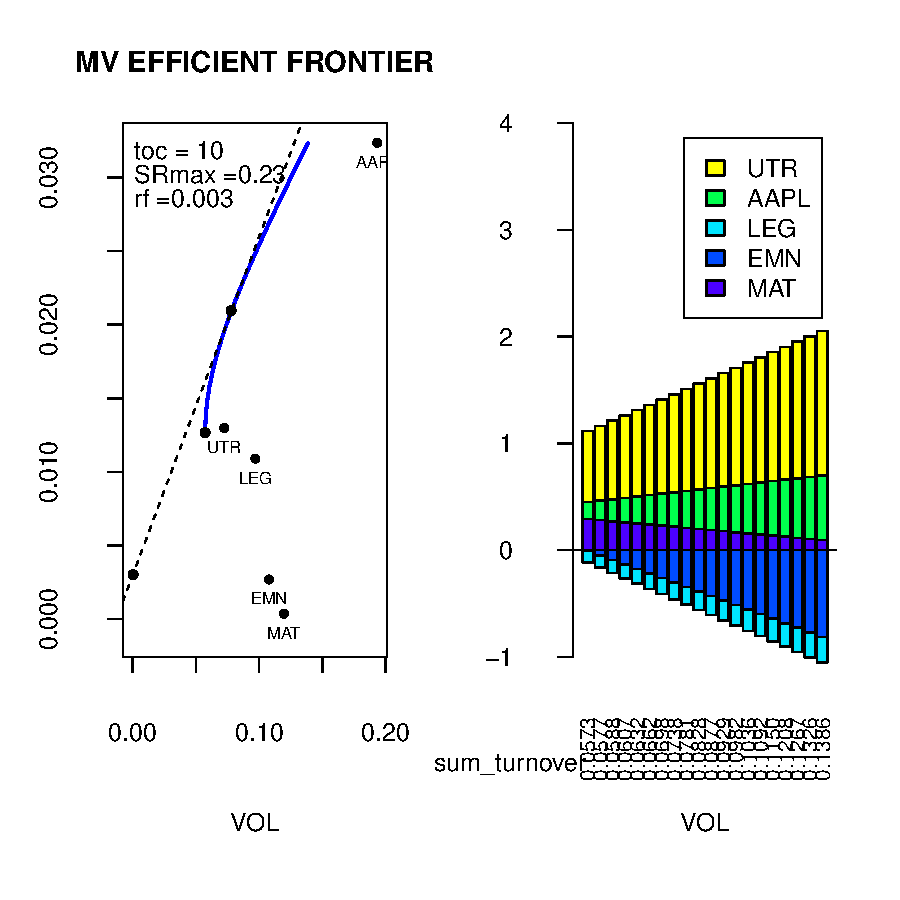
\includegraphics[width=\maxwidth]{figure/unnamed-chunk-71} 
\begin{kframe}\begin{alltt}

clist <- \hlkwd{c}(\hlstr{"sum"},\hlstr{"turnover.doug"})
list.arg <- \hlkwd{list}(	
		sum=sum,
		toc=toc,
		w.initial=w.initial)
cset <- NULL
cset <-\hlkwd{combine.cset}(clist=clist,returns=returns,list.arg)
\end{alltt}
\begin{verbatim}
## sum 
## turnover.doug
\end{verbatim}
\begin{alltt}

\hlkwd{efrontPlot}(returns, cset, rf = .003, npoints = 20,wts.plot = T,
		bar.ylim = \hlkwd{c}(-1,4),list.arg=list.arg)
\hlkwd{mtext}(\hlkwd{paste}(clist,collapse=\hlstr{"_"}),side=1,line=3)
\end{alltt}
\end{kframe}
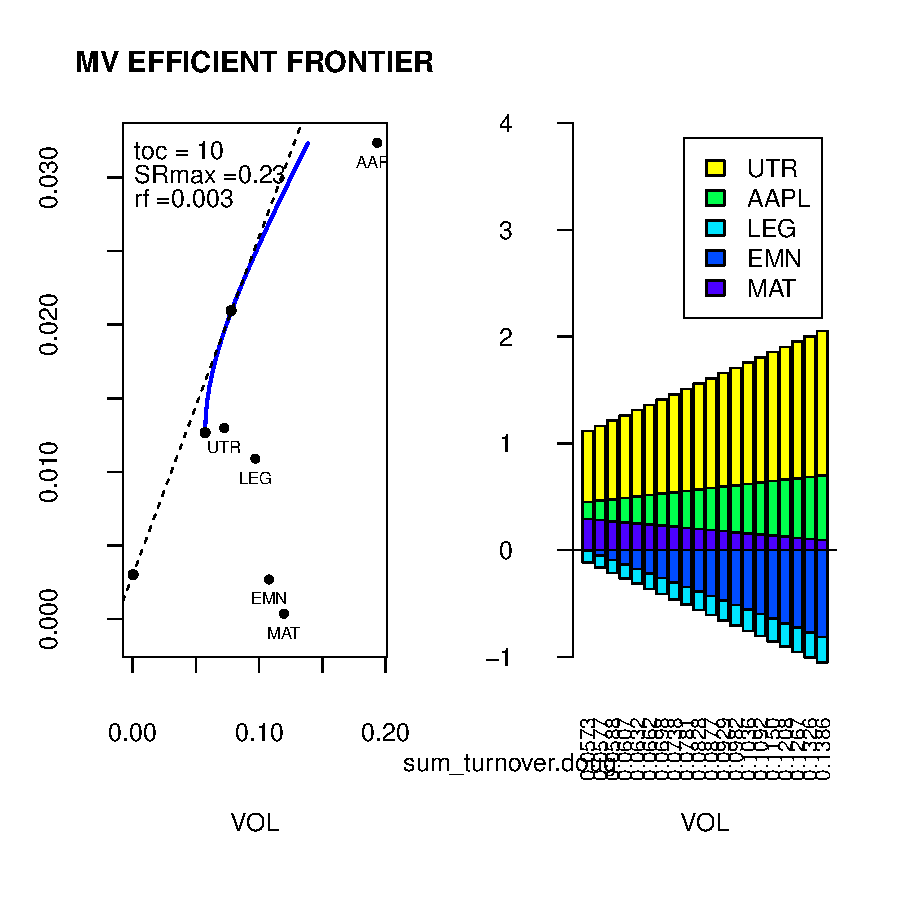
\includegraphics[width=\maxwidth]{figure/unnamed-chunk-72} 

\end{knitrout}



\end{document}
